\vspace{0.3cm}

\begin{itemize}

	\item[${\textbf{[G1]}}$] {\textbf{Allows a person to register and to have a personal area to which he/she can access with his/her credentials.}
		\begin{itemize}
			\item[$\textbf{[R1]}$] {A person can register in the application by providing his/her personal data, a unique e-mail and a password.}
			\item[$\textbf{[D1]}$] {The user has a device linked to his/her smartphone.}
			\item[$\textbf{[R2]}$] {A user can log in by providing his/her e-mail and password.}
			\item[$\textbf{[R3]}$] {Each user has a personal area associated with his/her credentials.
				\begin{itemize}
					\item[$\textbf{[R3.1]}$] {A user can see the third parties subscribed to his/her data in his/her personal area.}
					\item[$\textbf{[R3.2]}$] {A user can add weight and height in his/her personal area.}
					\item[$\textbf{[R3.3]}$] {A user can link his/her device to the app in his/her personal area.}
				\end{itemize}}
		\end{itemize}}


	\item[${\textbf{[G2]}}$] {\textbf{Allows the third party to register and to have a personal area to which it can access with his/her credentials.}
		\begin{itemize}
			\item[$\textbf{[R4]}$] {A third party can register in the application by providing his/her third party data, a unique e-mail and a password.}
			\item[$\textbf{[R5]}$] {A third party can log in by providing his/her e-mail and password.}
			\item[$\textbf{[R6]}$] {Each third party has a personal area associated with his/her credentials.
				\begin{itemize}
					\item[$\textbf{[R6.1]}$] {A third party can see the data of users and groups of users obtained from his/her personal area.}
					\item[$\textbf{[R6.2]}$] {A third party can require data to users or groups of users from his/her personal area.}
				\end {itemize}}
		\end{itemize}}


	\item[${\textbf{[G3]}}$] {\textbf{Allows the third party to require data.}
		\begin{itemize}
			\item[$\textbf{[D2]}$] {The user's smartphone can provide an accurate enough current location.}
			\item[$\textbf{[D3]}$] {The user's device can provide accurate enough healt parameters.}
			\item[$\textbf{[D4]}$] {The user's smartphone can provide constantly data to \hbox{\emph{D4H}}.}
			\item[${\textbf{[G3.1]}}$] {\textbf{Third party can require single person's data.}
				\begin{itemize}
					\item[$\textbf{[R7]}$] {A third party can require user's data by providing his/her fiscal code and the reason of the request.}
				\end{itemize}}
			\item[${\textbf{[G3.2]}}$] {\textbf{Third party can require anonymized data of group of people.}
				\begin{itemize}
					\item[$\textbf{[R8]}$] {A third party can require anonymized data of groups of users by providing constraints that define users.
						\begin{itemize}
							\item[$\textbf{[R8.1]}$] {The group of user to which require data can be specified by any combination of geographic areas, range of ages, 									sex, range of weights and range of heights.}
							\item[$\textbf{[R8.2]}$] {Requests of data related  to groups of users are accepted by \hbox{\emph{TrackMe}} if and only if the amount of 									users which respect the given constraints is equal or grater than 1000.}
						\end{itemize}}
				\end{itemize}}
		\end{itemize}}


	\item[${\textbf{[G4]}}$] {\textbf{Allows the user to accept or not to let a third party to have access to his/her/her data.}
		\begin{itemize}	
			\item[$\textbf{[R9]}$] {A user is notified by the \hbox{\emph{D4H}}'s app when a third party makes a request to have access to the user's data.}
			\item[$\textbf{[R10]}$] {A user can reply to a third party interested to his/her data from his/her personal area within 30 days.}
		\end{itemize}}


	\item[${\textbf{[G5]}}$] {\textbf{Allows third party to subscribe for new data.}
		\begin{itemize}
			\item[$\textbf{[R11]}$] {After a request has been accepted, the third party can decide to subscribe to the data of that user or group of users.}
			\item[$\textbf{[R12]}$] {A user is notified by the \hbox{\emph{D4H}}'s app when a third party decides to subscribe for his/her data.}
			\item[$\textbf{[R13]}$] {A user can stop the subscribe to his/her data by a third party in any moment from his/her personal area.}
			\item[$\textbf{[R14]}$] {If a user stops the subscribe of a third party to his/her data, the third party will be notified by the \hbox{\emph{D4H}}'s app.}
		\end{itemize}}


	\item[${\textbf{[G6]}}$] {\textbf{Allows third party to see users' or groups of users' data obtained through a successful request.}
		\begin{itemize}
			\item[$\textbf{[R15]}$] {Third parties can see the obtained data directly on their personal area.}
			\item[$\textbf{[R16]}$] {Third parties are notified by the \hbox{\emph{D4H}}'s app if their's request for new data has been rejected.}
		\end{itemize}}

	\item[${\textbf{[G7]}}$] {\textbf{Allows users to monitor their healt parameters.}}
		\begin{itemize}
			\item[$\textbf{[R20]}$] {A user can see his/her health parameters in his/her personal area.}
		\end{itemize}

	\item[${\textbf{[G8]}}$] {\textbf{Allows users to activate or deactivate the \hbox{\emph{ASOS}} service on top of \hbox{\emph{D4H}}.}
		\begin{itemize}
			\item[$\textbf{[R17]}$] {Users can activate or deactivate the \hbox{\emph{ASOS}} service from their's personal area.}
		\end{itemize}}


	\item[${\textbf{[G9]}}$] {\textbf{Allows an unhealty user to receive quick help if have the \hbox{\emph{ASOS}} service activated on his/her account.}
		\begin{itemize}
			\item[$\textbf{[D5]}$] {There is an SOS service that has the capability to receive emergency calls by \hbox{\emph{ASOS}}.
				\begin{itemize}
					\item[$\textbf{[D5.1]}$] {The SOS service has the capability to receive data about the unhealty user.}
					\item[$\textbf{[D5.2]}$] {The SOS service has the capability to send assistance to the unhealty user.}
				\end{itemize}}
			\item[$\textbf{[R18]}$] {ASOS is able to contact the SOS service in case of the rise of an unhealty user in 5s.}
			\item[$\textbf{[R19]}$] {ASOS is able to send to the SOS service the unhealty user's data and personal data.}
		\end{itemize}}
\end{itemize}

\subsection{Use Cases}
\def\A {Name}
\def\B {Actors}
\def\C {Entry conditions}
\def\D {Event Flow}
\def\E {Exit conditions}
\def\F {Exceptions}
\def\G {Goals}
\def\H {Requirements}

\renewcommand{\arraystretch}{1.5}

\begin{figure}[h!]
	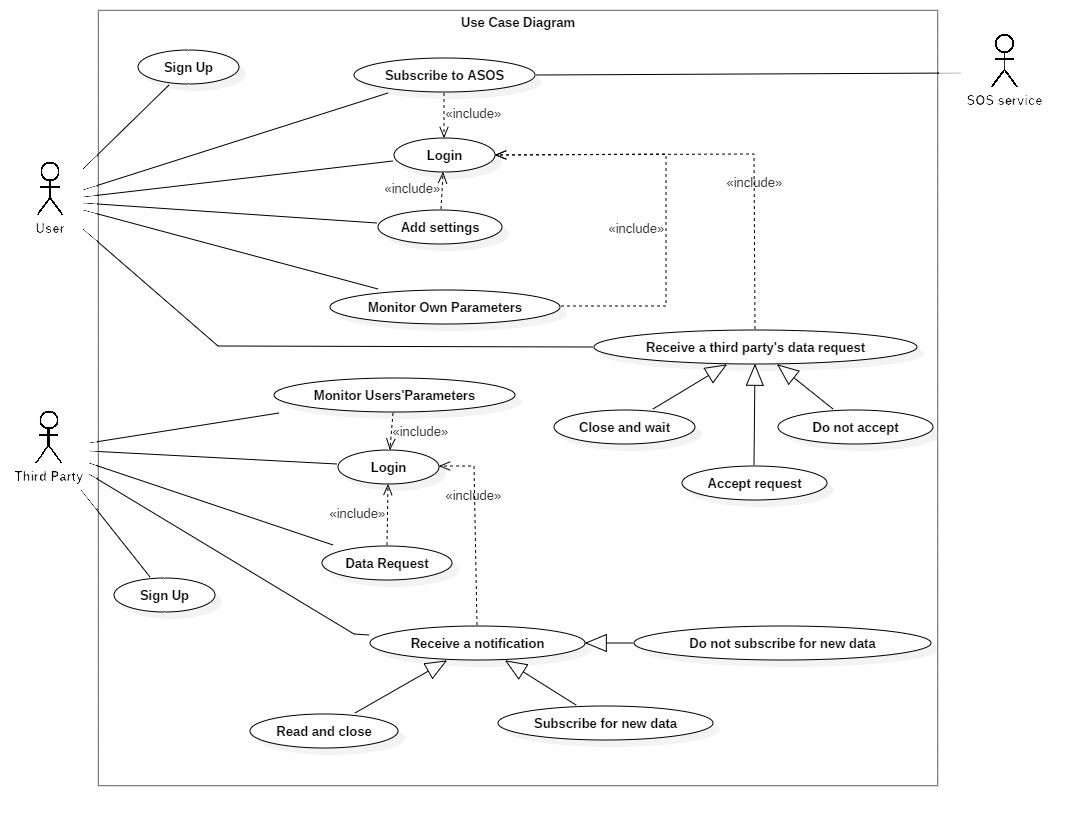
\includegraphics[width=1.1\textwidth]{./pictures/usecase_diagram.png}\par
	\caption{Figure 1: Use Case Diagram}
\end{figure}

\FloatBarrier

\subsubsection{Sign up}
\begin{center}
	\begin{longtable}{ | p{0.3\textwidth} | p{0.7\textwidth} | }
		\hline 
		 \A &  Sign Up \\ 

		\hline
		 \B &  User - Third party \\  %è da dividere?? sono necessari due diversi use cases??

		\hline
  		 \C &  The individual or the third party has downloaded the app on his/her smartphone.\\ 

		\hline
		 \D & \begin{enumerate}
			\item The individual opens the app on his/her smartphone;
			\item He/she clicks on the \textit{Register here} link;
			\item The user fills all the mandatory fields and provide all his/her personal data;
			\item He/she clicks on "Register" button;
			\item The system saves all personal data and creates a new personal area.
		\end{enumerate} \\

		\hline
		 \E &  The user has a personal area and now he/she is able to use the application.\\

		\hline
		 \F & \begin{enumerate}
			\item The user is already signed up
			\item The user didn’t fill all of the mandatory fields;
			\item The e-mail has already been registered;
			\item All the exceptions are handled by notifying the user and taking him back to the sign up activity.
		\end{enumerate} \\
		
		\hline
		 \G &  G1 - G2\\

		\hline
		 \H &  R1 - R3- R4 - R6 \\
		\hline

	\end{longtable}
\end{center}

\subsubsection{Login}
\begin{center}
	\begin{longtable}{ | p{0.3\textwidth} | p{0.7\textwidth} | }
		\hline
		 \A &   Login \\ 

		\hline
		 \B &  User - Third party \\ 

		\hline
  		 \C &  The user or the third party has the application installed; has succesfully registered and has a personal area.\\ 

		\hline
		\D & \begin{enumerate}
			\item The user  or the third party opens the app on his/her smartphone;
			\item Writes his/her credentials;
			\item Clicks on "Login" button;
		\end{enumerate} \\

		\hline
		\E & The user  or the third party is succesfully redirected to his/her main page.\\

		\hline
		\F & \begin{enumerate}
			\item The user or the third party doesn't register yet;
			\item The user or the third party enters an invalid Username;
			\item The user or the third party enters an invalid Password;
			\item He/she doesn't fill all fields.
		\end{enumerate} All the exceptions are handled by notifying the user and taking him/her back to the login activity. \\
		
		\hline
		\G & G1 - G2\\

		\hline
		\H & R2 - R3.1- R5 - R6.1 \\
		\hline

	\end{longtable}
\end{center}

\subsubsection{Add settings details}
\begin{center}
	\begin{longtable}{ | p{0.3\textwidth} | p{0.7\textwidth} | }
		\hline
		 \A &   Add settings details\\ 

		\hline
		 \B &  User \\ 

		\hline
  		 \C &  The user has the application installed; has successfully registered; has a personal area and has a device that can be linked to the smartphone.\\ 

		\hline
		\D & \begin{enumerate}
			\item The user opens the app on his/her smartphone;
			\item He/she login;
			\item Opens the Menu by the three points icon in the main scene;
			\item Clicks on the \textit{Settings} link;
			\item Inserts his/her weight and height;
			\item Adds his/her device;
			\item Clicks the \textit{Save} button.
		\end{enumerate} \\

		\hline
		\E & The app saves successfully all personal data and the device starts to send health parameters.\\

		\hline
		\F & \begin{enumerate}
			\item The user exits from the Settings area without saving, this exception is handled by notifying it to the user;
			\item The user doesn't link any personal device, this exception can't be handled but the user notices it because 					without a linked device the app can't run correctely.
		\end{enumerate} \\
		
		\hline
		\G & G1\\

		\hline
		\H & R3.1 - R3.3 \\
		\hline

	\end{longtable}
\end{center}

\subsubsection{Monitor own parameters}
\begin{center}
	\begin{longtable}{ | p{0.3\textwidth} | p{0.7\textwidth} | }
		\hline
		 \A &  Monitor his/her own parameters\\ 

		\hline
		 \B &  User \\ 

		\hline
  		 \C &    The user has the application installed; has succesfully registered; has a personal area, has added settings details and has a device linked to his/her smartphone.\\

		\hline
		\D & \begin{enumerate}
			\item The user login;
		\end{enumerate} \\

		\hline
		\E & The app opens the main scene in which the user can see his/her health paramters by graphs and numbers.\\

		\hline
		\F & - \\
		
		\hline
		\G & G7\\

		\hline
		\H & R20\\
		\hline

	\end{longtable}
\end{center}

\subsubsection{Receive a third party's data request}
In the figure 3.21 there are three use cases which derives from this abstract one; their difference is given by the last step of the event flow and the exit condition. Because of this reason we have chosen to compress them in just one table.
\begin{center}
	\begin{longtable}{ | p{0.3\textwidth} | p{0.7\textwidth} | }
		\hline
		 \A &   Receive a notification\\ 

		\hline
		 \B &  User \\ 

		\hline
  		 \C &  The user has the application installed; has succesfully registered; has a personal area and has a device linked to his/her smartphone.\\ 

		\hline
		\D & \begin{enumerate}
			\item The user receives a notification on his/her smartphone;
			\item He/she login and finds an alert;
			\item Reads the alert;
			\item Click on the \textit{Accept} button or on the \textit{Refuse} button or on the \textit{Exit} icon.
		\end{enumerate} \\

		\hline
		\E & The allert is closed and the choise is saved: \begin{enumerate}
			\item if he/she has clicked on the \textit{Exit} icon the notification is added in the \textit{Data Request Notification} 				area;
			\item if he/she has clicked on the \textit{Accept} button the third party is added in the \textit{Third Party} area;					\item else it is delated.
		\end{enumerate}\\

		\hline
		\F & \begin{enumerate}
			\item The user doesn't accept neither refuse before the time bound.
		\end{enumerate} This exception is resolved by considering the non answer as a negative one. \\
		
		\hline
		\G & G4\\

		\hline
		\H & R3.2 - R9 - R10 \\
		\hline

	\end{longtable}
\end{center}

\subsubsection{Receive a notification (third party)}
In the figure 3.21 there are three use cases which derives from this abstract one; their difference is given by the last step of the event flow and the exit condition. Because of this reason we have chosen to compress them in just one table.
\begin{center}
	\begin{longtable}{ | p{0.3\textwidth} | p{0.7\textwidth} | }
		\hline
		 \A &   Receive a notification\\ 

		\hline
		 \B &  Third Party \\ 

		\hline
  		 \C &  The third party has the application installed; has succesfully registered and has a personal area.\\ 

		\hline
		\D & \begin{enumerate}
			\item The third party receives a notification;
			\item The third party login and finds an alert;
			\item Reads the alert;
			\item Clicks on the \textit{Subscribe} button or on the \textit{Refuse} button or on the \textit{Exit} icon.
		\end{enumerate} \\

		\hline
		\E & The allert is closed and the choise is saved: \begin{enumerate}
			\item if the third party  has clicked on the \textit{Subscribe} button the single user data or the group of users data are 				added in the main scene and the third party will always receive new data ;					
			\item  if the third party  has clicked on the \textit{Refuse} button the single user data or the group of users data are 				added in the main scene and the third party won't receive new data ;	
			\item else nothing happens.
		\end{enumerate}\\

		\hline
		\F & -\\
		\hline
		\G & G5 - G6\\

		\hline
		\H & R6.1 - R11 - R12 - R13 - R14 - R15 - R16\\
		\hline

	\end{longtable}
\end{center}

\subsubsection{Subscribe to \textit{ASOS}}
\begin{center}
	\begin{longtable}{ | p{0.3\textwidth} | p{0.7\textwidth} | }
		\hline
		 \A &   Subscribe to \textit{ASOS}\\ 

		\hline
		 \B &  User \\ 

		\hline
  		 \C &  The user has the application installed; has succesfully registered; has a personal area and has a device linked to the smartphone.\\ 

		\hline
		\D & \begin{enumerate}
			\item He/she login;
			\item Opens the menu and clicks on the \textit{ASOS} link;
			\item Checks the check boxes;
			\item Clicks on the \textit{Save} button.
		\end{enumerate} \\

		\hline
		\E & The app saves the choise and activate the \textit{ASOS} service.\\

		\hline
		\F & - \\
		
		\hline
		\G & G7 - G8\\

		\hline
		\H & R17 - R18 - R19 \\
		\hline

	\end{longtable}
\end{center}

\subsubsection{Data request}
\begin{center}
	\begin{longtable}{ | p{0.3\textwidth} | p{0.7\textwidth} | }
		\hline
		 \A &  Request data\\ 

		\hline
		 \B &  Third Party \\ 

		\hline
  		 \C &  The third party has the application installed; has succesfully registered and has a personal area.\\

		\hline
		\D & \begin{enumerate}
			\item The third party login;
			\item Clicks on the plus icon in the main scene: if the request is for single user data the first one else the second;
			\item Fills all the mandatory fields with the required data  ;
			\item Clicks on the \textit{Save and Send request} button.
		\end{enumerate} \\

		\hline
		\E & The app saves the request and starts to elaborate it.\\

		\hline
		\F & \begin{enumerate}
			\item The third party doesn't fill any field.
		\end{enumerate} The exception is handled by notifying the third party and taking him back to the Request Data activity. \\
		
		\hline
		\G & G3 - G3.1 - G3.2\\

		\hline
		\H & R6.2 - R7 - R8 - R8.1 \\
		\hline

	\end{longtable}
\end{center}

\subsubsection{Monitor users' parameters}
\begin{center}
	\begin{longtable}{ | p{0.3\textwidth} | p{0.7\textwidth} | }
		\hline
		 \A &  Monitor users' parameters\\ 

		\hline
		 \B &  Third Party \\ 

		\hline
  		 \C &  The third party has the application installed; has succesfully registered; has a personal area and has received data of some single users and some group of users.\\

		\hline
		\D & \begin{enumerate}
			\item The third party login;
			\item Clicks on a \textit{Fiscal code X} button or on a \textit{Group X} button;
		\end{enumerate} \\

		\hline
		\E & The app opens the health parameter of the user associated to the clicked fiscal code or to the group of users associated to the considered group.\\

		\hline
		\F & - \\
		
		\hline
		\G & G6\\

		\hline
		\H & R6.1 - R15 \\
		\hline

	\end{longtable}
\end{center}
\subsection{Sequence Diagrams}
In this section are reported the most meaningful sequence diagrams in relation to some scenarios previously presented.

\begin{figure}[!h]
	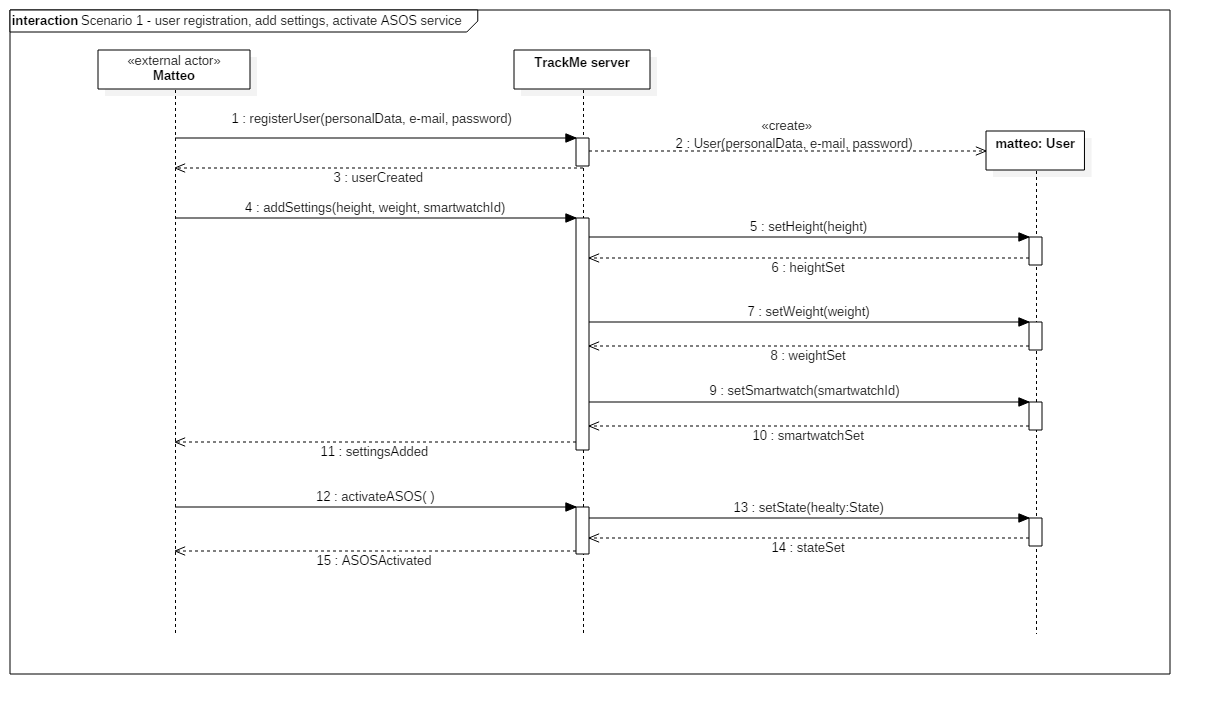
\includegraphics[width=1.00\textwidth]{./pictures/Scenario_1.png}\par
	\caption{Figure 1: Sequence diagram relative to the scenario 1.}
\end{figure}
\FloatBarrier
\vspace{0.3cm}

\begin{figure}[!h]
	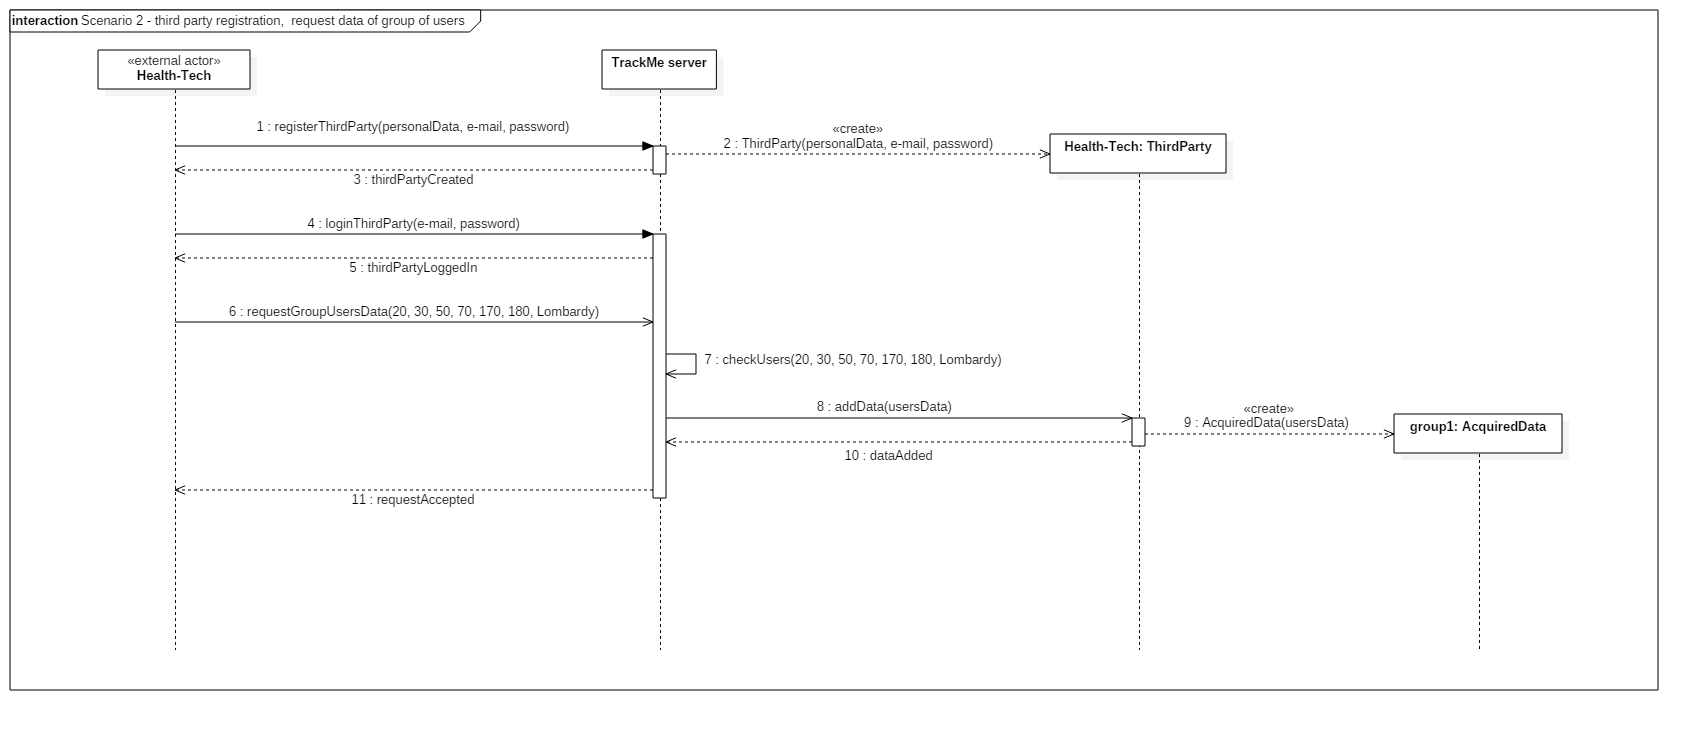
\includegraphics[width=1.00\textwidth]{./pictures/Scenario_2.png}\par
	\caption{Figure 2: Sequence diagram relative to the scenario 2.}
\end{figure}
\FloatBarrier
\vspace{0.3cm}

\begin{figure}[!h]
	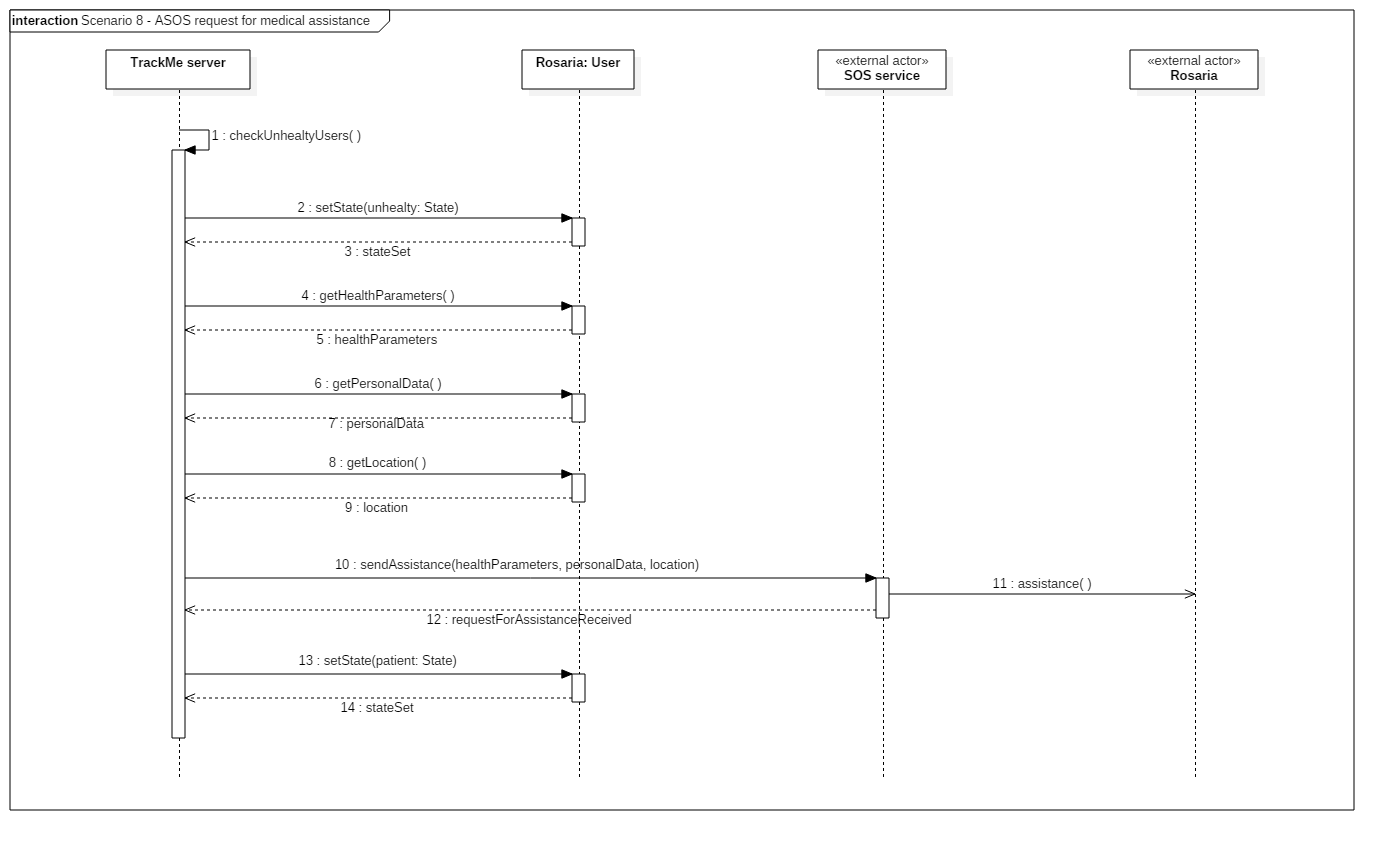
\includegraphics[width=1.00\textwidth]{./pictures/Scenario_8.png}\par
	\caption{Figure 3: Sequence diagram relative to the scenario 8.}
\end{figure}
\FloatBarrier
\vspace{0.3cm}
